\documentclass[12pt, fleqn]{article}

\usepackage{../../../template/template}

\begin{document}
\begin{lect} {Метрические пространства \q 2019-09-04} 
	\[M \q d: M \times M \rightarrow [0; +\infty)\]
	d - метрика
	\begin{theorem} {Аксиомы метрики:}
			\begin{enumerate}
				\item \[d(x, y) \geq 0\]
				\item \[d(x, y) = 0 \rla x = y\]
				\item \[d(x, y) = d(y, x)\]
				\item \[d(x, y) \leq d(x, z) + d(z, y)\]
			\end{enumerate}
	\end{theorem}
	\begin{examples}
		\begin{enumerate}
			\item \[M = \R^n \q x \in M \q x = (x_1, ..., x_n)\]
				\[d_{\infty}(x,y) = \max_{1 \leq j \leq n}|x_j - y_j|\]
			\item \[M = \R^n,\]
			\[d_p(x,y) = \sqrt[p]{\sum{|x_j - y_j|}^n_{j = 1}}\]
			\[\text{В частн. } d_2(x, y) = \sqrt{\sum^n{|x_j - y_j|^2}\]
			\item \[M = C[0,1]\]
				\[f, g \in M\]
				\[d(f, g) = \sup_{x \in [0, 1]}|f(x) - g(x)| \]
			\item \[M = C[-1, 1] \q d(f, g) = \int_{-1}^1 |f-g| \]
		\end{enumerate}
	\end{examples}
	\begin{utv}
		\[\max_{1 \leq j \leq n}|x_j - y_j| \leq \sqrt{\sum^n_{j = 1}{|x_j - y_j|^2}} 
		\leq n \cdot \max_{1 \leq j \leq n} |x_j - y_j|\]
		\[d_{\infty}(x, y) \leq d_2(x, y) \leq n \cdot d_{\infty}(x, y)\]

	\end{utv}
	\begin{definition}
		\[x^{(m)} \in M\]
		\[\lim_{m \to \infty} x^{(m)} = x \rla d(x^{(m)}, x) \underset{m \to \infty}{\to}0\]
	\end{definition}
	\begin{example}
		\begin{enumerate}
			\item \[M = C[0, 1] \q d(f, g) = \sup_{x \in [0, 1]} |f(x) - g(x)|\]
				\[f^{(m)} \underset{d}{\to} f \rla f^{(m} \underset{[0, 1]}{\rightrightarrows} f\]
			\item \[M = \R^n, d_2(x, y) \q x^{(m)} = (x_1^{(m)},  ..., x_n^{(m)})\]
				\[\text{сх-сть } (\R^n, d_2) \rla \text{ покоорд сх-ти}\]
				\[x^{(m)} \underset{d_2}{\to} x \rla x^{(m)}_j \to x_j \q \forall j = 1,...n\]
		\end{enumerate}
		Т.о сх-ть по метрике $d_2$ в $\R^n$ равносильна покоорд сх-ти
	\end{example}
	\begin{theorem}[Критерий Коши]
		\[(\R^n, d_2)\]
		\[x^{(m)} \underset{m \to \infty}{\to} x \rla \forall \mathcal{E} > 0 \exists N: \forall n, k \geq N \]
		\[d_2(x^{(n)}, x^{(k)}) < \mathcal{E} \text{ (УПР)}\]

		Аналогичн. Т. Верна не для всех метрич. пр-в:
		\[\text{Напр: } M = C[-1, 1] \q d(f, g) = \int_{-1}^1 |f-g|\]
		\[f_n:\]
		\begin{figure}[h]
		    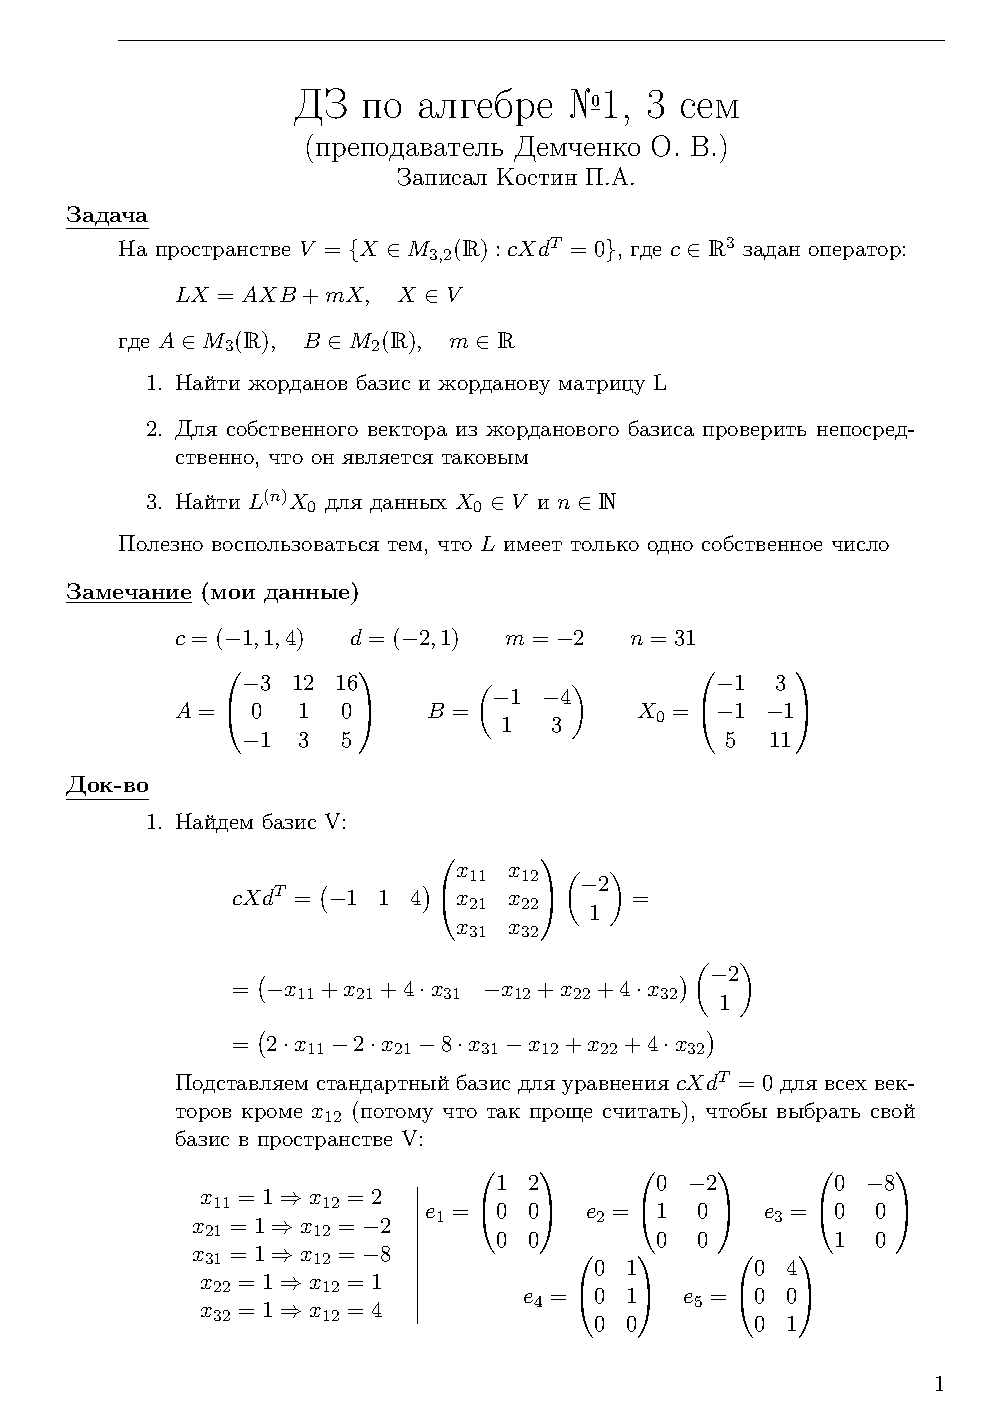
\includegraphics[scale=0.5]{pics/1.jpg}
		    \centering
		\end{figure}
		
		\[\{f_n\} \text{ - сх. в себе: }\]
		\[\forall \mathcal{E} > 0 \exists N: \forall n > N \ \forall p > 0 ?\]
		\[d(f_n, f_{n + p}) < \mathcal{E}\]
		\[d(f_n, f_{n + p}) = \int_{-1}^1 |f_n - f_{n + p}| = \frac{1}{n} - \frac{1}{n + p} \leq \frac{1}{n} \to 0 \]
			\[\forall \mathcal{E} \exists N: \forall n > N, p > 0 \ d(f_n, f_{n + p}) < \mathcal{E}\]
		\begin{figure}[h]
			\includegraphics[scale=0.5]{pics/2.jpg}\\
			\centering		
		\end{figure}
		
		Усл. Коши удовл. (сх в себе)
		\[\text{Есть ли } \lim_{n \to \infty} f_n ? \]
		\[g(x) = sign \ x \text{ поточечн предел}\]
		\[\lim_{n \to \infty} \int_{-1}^1 |f_b - g| = 0 \text{, но } g \not \in C[-1, 1]\]
		\[\text{предпол } f \in C[-1, 1] \q \lim{f_n} = f \text{ т.е } \int |f_n - f| \to 0 \]
		\[0 \leq \int_{-1}^1|f-g| \leq \int_{-1}^1 |f_n - f| + \int_{-1}^1 |f_n - g| \underset{n \to \infty}{\to} 0 \]
		\[\int_{-1}^1 \underset{\q \in C[-1; 1]}{ |f - g|} = 0\]
		\[\int_{-1}^0 \underset{= 0}{|f - g\mid} + \int_{0}^1 \underset{= 0}{|f - g|} \ra 
			\begin{align}
				&f(x) = 1 \q &\forall x > 0\\
				&f(x) = -1 \q &\forall x < 0
			\end{align}
		\]
		\[\text{ - неустранимый разрыв в т.} x = 0 \q \ra \lim f_n \text{ не существует} \]
		\[\text{УПР } C[0, 1] \q d(f, g) = \sup_{1 \leq x \leq y} |f(x) - g(x)|\]
		Вып ли Т. Коши?
	\end{theorem}
	Топология 
	\[\R^n \q d(x, y) = \sqrt{\sum_{j = 1}^n |x_j - y_j|^2}\]
	\[B(a, r) = \{x \in \R^n : d(a, x) < r\}\]
	\[X \subset \R^n \q X \text{ - откр, если }\]
	\[\forall a \in X \exists B_a : B_a \subset X\]
	\[X \text{ - замкн } \rla X^c \text{ - откр}\]
	\begin{theorem}[св-ва]
			\begin{enumerate}
				\item \[U_\alpha \text{ - откр } \forall \alpha \in A \ra \bigcup_{\alpha \in A} U_\alpha \text{ - откр. }\]
				\item \[\{U_k\}^N_{k = 1} \text{ - откр } \ra \bigcap_{k = 1}^n U_k \text{ - откр}\]
				\item \[F_\alpha \text{ - замк } \forall \alpha \in A \ra \bigcap_{\alpha \in A}F_\alpha\]
				\item \[F_k \text{ - замкн } \ra \bigcup_{k = 1}^N F_k \text{ - замк}\]
			\end{enumerate}
	\end{theorem}
	\begin{definition}
			Окр. т a - $U $ - откр: $ a \in U$\\
			$\delta	$ окр-ть т. a $U_a(\delta) = B(a, \delta)$\\
			прокол. $\delta $ окр-ть\\
			\[\doted{U_a}(\delta) = B(a, \delta) \setminus \{a\}\]
			Внутренность $X \subset \R^n$
			\[int(X) = \{a \in X: \exists B_a \subset X\}\]
			Внешность $X \subset \R^n$
			\[ext(X) = int(X^c) = \{b \in X^c : \exists B_b \subset X^c\}\]
			Замыкание
			\[Cl(X) = (ext(X))^c\]
			Граница
			\[\partial X = Cl(x) \setminus int(X) = \R^n \setminus (int X \cup ext X)\]
	\end{definition}
	\begin{examples}
		\[X = B(0, 1)\]
		\[int X = B(0, 1)\]
		\[ex X = \{x : d(0, x) > 1\}\]
		\[Cl X = \overline{B}(0, 1) = \{x : d(0, x) \leq 1\}\]
		Рисунок шарика
		\[\partial X = S(0, 1) = \{x : d(0, x) = 1\}\]
		УПР. Доказать или опровергнуть
		\begin{enumerate}
			\item \[int(int X) = int X\]
			\item \[\partial(\partial X) = \partial X\]
			\item \[Cl(Cl X) = Cl X\]
		\end{enumerate}
	\end{examples}
	\begin{utv}
			\[X \text{ - замкн } \rla Cl X = X\]
	\end{utv}
	\begin{proof}
		\[U \text{ - откр } \q int U = U\]
		\[\ra X \text{ - замкн } \rla X^c \text{ - откр.} \rla ext X = int(X^c) = X^c \rla  \]
		\[Cl X = (ext X)^c = X^{cc} = X\]
	\end{proof}
	\begin{definition}
		Ограниченность
		\[X \subset \R^n\]
		\[diam X = \sup_{x, y \in X} d(x, y)\]
		\[X \text{ - огр. если } diam X < \infty \rla \exists R > 0: X \subset B(0, R) \text{ (УПР)}\]
	\end{definition}
	\begin{theorem}[Принцип выбора Больцано-Вейерштр.]
		\[\forall \text{ огр. послед. } \{X^{(m)}\} \subset \R^n \text{ можно выделить сх. подпослед.
}\]
	\end{theorem}
	Компатные множества в $\R^n$
	\begin{definition}
			\[K \subset \R^n \text{ - компактное мн-во } \rla \forall \text{ откр. покр. можно выделить конеч. подпокр.}\]
			\[\text{Если } U_\alpha - \text{ откр .} \forall \alpha \in A : K \subset \bigcup_{\alpha \in A}U_\alpha \ra \exists \alpha_1, ..., \alpha_n \in A:\]
			\[K \subset \bigcup^N_{k = 1}U_\alpha\]
	\end{definition}
	\begin{examples}
			\begin{enumerate}
				\item \[[a, b] \subset \R \text{ - компакт.}\]
				\item \[I = \prod_{j = 1}^n [a_j, b_j] \subset \R^n\]
					\begin{figure}[h]
					    \includegraphics[scale=0.5]{pics/3}
					    \centering
					\end{figure}
					
				\[I_0 \supset I_1 \supset I_2 \supset ... \supset I_n\]
				\[diam I_n = \frac{diam I}{2^n} \to 0\]
				\[I_n \text{ - замк}\]
			\[I_k = \prod_{j = 1} ^n [a_j^{(k)}, b_j^{(k)} ]  \q\q \bigcap_{k \in \N} [a_j^{(k)}, b_j^{(k)}] = \{c_j\} \forall j \]
				\[[a_j^{(k)}, b_j^{(k)}] \supset [a_j^{(k+1)}], b_j^{(k+1)}\]
				\[x^* \in \bigcap_{k \in \N} I_k\]
				\[\text{Если } y^* \in \bigcap_{k \in \N} I_k \ra d(x^*, y^*) \leq diam I_k \to 0\]
				\[\ra d(x^*, y^*) = 0 \ra x^* = y^*\]

				\[x^* = \bigcap_{k = 1}^{\infty} I_k\]
				\[x^* \in I \subset \bigcup_{\alpha \in A} U_\alpha \ra \]
				\[\exists \alpha^* : x^* \in U_{\alpha^*} \text{ - откр}\]
				\[\exists B(x^*, \delta) \subset U_{\alpha^*}\]
				\[\ra \exists N \in \N : I_N \subset U_{\alpha^*}\]
			\end{enumerate}
	\end{examples}
\end{lect}
\begin{lect}
	\begin{lemma}
			\[K \subset \R^n \text{ - компакт }\]
			Тогда
			\begin{enumerate}
				\item K - замкн
				\item K - огр
				\item $\forall D \subset K \q D \text{ - замк } \ra D \text{ - комп} $ 
			\end{enumerate}
	\end{lemma}b	
	\begin{proof}
			\begin{enumerate}
				\item \[K^c \ni a \text{Рисунок области с k x a}\]
					\[\forall x \in K \q d(a, x) > 0\]
					\[r_x = \frac{1}{3} d(x, a)\]
					\[\forall x \in K\]
					\[B(x, r_x) \text{ - откр}\]
					\[K \subset \bigcup_{x \in K} B(x, r_x) \text{ - откр. покр. компакта } K\]
					\[\exists x_1, ..., x_N \in K : K \subset \bigcup_{j = 1}^N B(x_j, r_{x_j})\]
					\[a \in \bigcap_{k = 1}^N B(a, r_{x_k}) = B(a, r_{\min}\]
					\[r = \min(r_x, r_{x_N}) > 0\]
					\[\text{ причем } \bigcap_{1}^N B(a, r_{x_k}) \text{ не имеет общих точек}\]
					\[\bigcup_{1}^N B(x_k, r_{x_k})\supset K\]
					\[\exists B(a, e_{mn}) \subset K^c \ra K^c \text{ - откр }\ra \text{K - замкн} \]

				\item \[ \text{комп - }K \subset \bigcup_{k = 1}^\infty B(0, k) \text{ - откр. покр} \]
					\[\ra \exists k_1, ..., k_n\]
					\[K \subset \bigcup_{j = 1}^N B(0, k_j) = B(0, \max_{1 \leq j \leq N}(k_j)) \ra K \text{ - огр} \]
				\item \[\text{замкн - }D \subset K \text{ - комп}\]
					Пусть откр. покр
					\[D \subset \bigcup_{\alpha \in A} U_\alpha \]
					\[U^* = D^c \text{ - откр - добавим к покр. K} \{U_\alpha\}_{\alpha \in A}\]
					\[\ra \text{ выд. конечн. подпокрытие } K \q \{U_{\alpha_j}\}_{j = 1}^N \cup \{U^*\} \]
					\[D \subset \bigcup_{j = 1}^N U_\alpha\]
			\end{enumerate}
	\end{proof}
	\begin{theorem}[След. усл. равносильны]
			\begin{enumerate}
				\item K - компакт.
				\item K - замк. и огр.
				\item \[\forall \{x_m\}_{m = 1}^\infty \ x_m \in K\]
					\[\exists \text{ подпосл } x_{m_k} \to x \in K\]
			\end{enumerate}
	\end{theorem}
	\begin{proof}
			$1 \ra 2$\\
			$2 \ra 1$
			\[\text{т.к. } K \text{ - огр} \ra \exists I = \prod_{j = 1}^n [a_j, b_j]\]
			\[\text{замкн - }K \subset I \text{ - комп}\]
			$\ra$ (лемма) K - комп\\
			$2 \ra 3$
			\[x_m \in K \text{ - замк и огр}\]
			\[\ra \exists x_{m_k} \text{ - сх (пр. выб. Б-В)}\]
			\[x_{m_k} \to x \text{ предпол } x \not \in K\]
			\[x \in K^c \text{ - откр } \ra \exists B_x \subset K^c\]
			\[\text{Но } K \ni d(x_{m_k}, x) \to 0 \text{ противореч } x \in K \]
			$3 \ra 2$
			\[\text{а) предп.} K \text{ не явл. огр.} \]
			\[\forall n \in \N \q \exists x_n \in K: d(0, x_n) > n\]
			\[\{x_n\} \text{ не огр} \ra \text{ не сх.}\]
			\[\ra K \text{ - огр}\]
			\[\text{б) предп., что } K \text{ - не явл. замкн}\]
			\[K^c \text{ - не откр }\]
			\[\exists a \in K^c : \forall \delta > 0 \  B(a, \delta) \cap K \neq \varnothing\]
			\[\exists x_n \in B(a, \frac{1}{n}) \cap K\]
			\[x_n \in K\]
			\[0 \leq d(x_n, a) < \frac{1}{n} \to 0 \q x_n \to a; \ x_{n_k} \to x \in K\]
			\begin{figure}[h]
			    \includegraphics[scale=0.5]{pics/4}
			    \centering
			\end{figure}
			


			УПР: \[K_1 \supset K_2 \supset ...\]
			\[\text{д-ть } \bigcap_{j \in \N} K_j \neq \varnothing\]
		\end{proof}
		
		\begin{definition}
				Отображения в $\R^n$
				\[E \subset \R^n\]
				\[f: E \to \R^m \text{ - отобр-е (вект. ф-я)}\]
				\[m = 1 \text{ - ф-я}\]
				\[f(x) = (f_1(x), ..., f_m(x))\]
				\[= (x_1, ..., x_n) \q f_j: E \to \R \text{ коорд. функ-ии}\]
				\[a \in \R^n\]
				\[a \text{ - пред. т. E, если }\]
				\[\forall \delta > 0 \q U()(a, \delta) \cap E \neq \varnothing\]
		\end{definition}
		\begin{definition}
				\[f: E \to \R^m, a \text{ - пред. т E}\]
				\[\lim_{x \to a} f(x) = L \text{, если}\]
				\[\text{(Коши }) \forall \mathcal{E} > 0 \exists \delta > 0 : \forall x \in E\]
				\[0 < d(x, a) < \delta \ra d(f(x), L) < \mathcal{E}\]
				\[\text{(Гейне) } \forall \{x_k\}_{k = 1}^\infty \q x_k \in E \setminus \{a\} x_k \to_{k \to \infty} a  \ra F(x_k) \to_{k \to \infty} L \]
		\end{definition}
		\begin{example}
			\[f(x, y) = \left\{ \begin{align}
					&\frac{xy}{x^2 + y^2}, & (x,y) \neq (0, 0)\\
					&0, & (x,y) = (0, 0)
			\end{align}\]
			Повторные пределы
			\[\lim_{x \to 0} \lim_{y \to 0} f(x, y) = 0\]
			\[\lim_{y \to 0} \lim_{x \to 0} f(x, y) = 0 \]
			\[f(\delta, \delta) = \frac{1}{2} \underset{\delta \to 0}{\to}\frac{1}{2}\]
			\begin{figure}[h]
			    \includegraphics[scale=0.5]{pics/5}
			    \centering
			\end{figure}
			
			\[f(\delta, -\delta) = -\frac{1}{2}\]
			\[\text{т.е } \lim_{(x, y) \to (0,0)} f(x, y) \text{ не сущ.} \]
		\end{example}

		\begin{theorem}[предел композиции]
				\[E \subset \R^n, \q F \subset \R^m \q\q \R^n \ni a \text{ - пред т. E} \ F \ni b \text{ - пред. т. F}\]
				\[f: E \to F; \q g: F \to \R^l\]
				\[\lim_{x \to a} f(x) = b; \q \lim_{x \to b} g(x) = g(b) \]
				\begin{figure}[h]
				    \includegraphics[scale=0.5]{pics/6}
				    \centering
				\end{figure}
				
				\[\text{ Тогда } \lim_{x \to a} g \circ f = g(b) \]
		\end{theorem}
		\begin{theorem}[Крит. Коши]
				\[a \text{ - пред т. } E\]
				\[f(x) \text{ имеет предел в т.} a\]
				\[ \rla \forall \mathcal{E} > 0 \exists \delta > 0 : 
				\forall x, y \in \doted{U}(a, \delta) \cap E \ra d(f(x), f(y)) < \mathcal{E}\]
		\end{theorem}
		\begin{definition} [непрерывные отоб-я]
				\[a \in E \q\q f: E \to \R^m\]
				Если $a$ - изол $\ra f$ - непр в $a$,\\
				если $a$ - пред, то $f \text{ - непр в т. } a \rla $\\
				\[\rla \lim_{x \to a}f(x) = f(a) \]
				\[f \text{ - непр в т.} a \rla f_j \text{ - непр. в т } a \ \forall 1 \leq j \leq m\]
				\[f \text{ - непр в т. } a; g \text{ - непр в } f(a) \rla g \circ f \text{ - непр в т } a\]
				\[\text{непр сохр. при +, умн. на число}\]
				\[f \text{ - непр на } E \rla \text{ непр } \forall a \in E\]
		\end{definition}
		\begin{theorem}
				\[f: E \to \R^m\]
				\[f \text{ - непр на } E \rla \forall G \subset \R^m \q G \text{ - откр } \ra 
				f^{-1}(G) \text{ - откр в } E\]
		\end{theorem}
		\begin{proof}
			\[G \text{ - откр.}\]
			\[f^{-1}(G) \text{ - откр ?}\]
			\[a \in f^{-1}(G)\]
			\[f(a) \in G \text{ - откр } \ra \exists U(f(a), \mathcal{E}) \subset G\]
			рисунок
			\[\text{т.к } f \text{ непр в т. } a \]
			\[\exists \delta : d(a, x) < \delta \ra d(f(a), f(x)) < \mathcal{E}\]
			\[f(B(a, \delta)) \subset B(f(a), \mathcal{E}) \subset G\]
			\[\ra B(a, \delta) \subset f^{-1}(G)\]
			\[\la a \in E \ra ? f \text{ - непр в т. a} \text{ (рисунок)}\]
			\begin{figure}[h]
			    \includegraphics[scale=0.5]{pics/7}
			    \centering
			\end{figure}
			
			\[\forall \mathcal{E} > 0 B(f(a), \mathcal{E}) \text{ - откр в } \R^m\]
			\[\ra f^{-1}(B(f(a), \mathcal{E}) \text{ - откр.} \ra \exists \delta : B(a, \delta) \subset f^{-1}
			(B(f(a), \mathcal{E})) \ra f \text{ - непр. в т } a\]
			
		\end{proof}
		\begin{theorem}[локальные свойства непр. функций]
			\begin{enumerate} (дописать)
					\item непрерывна в т. a $\ra$ найдетс
					\item f непр в a.; g непр в a, $f \circ g$ непр в a. 
				\end{enumerate}
		\end{theorem}
\end{lect}
\end{document}






















